\chapter{Bewertung}

\section{Handschuh Qualität}

Die Sensoren liegen fest auf den Fingern und werden auch bei schnellerer Bewegung nicht lose. Sie können auch durch ihre austauschbaren und anpassbare Fingerhalterungen auf die eigene Fingerlänge oder Größe angepasst werden und gibt somit größeren Spielraum für den Komfort. Durch das anbringen des MPU-9250 auf dem Multiplexer ist dieser sehr anfällig auf Fehler, da die Kabel verbunden mit den IMUs den Multiplexer mit bewegen, welches auch den MPU-9250 beeinflusst. 
Die drahtlose Verbindung wirkt sich positiv auf den Bewegungskomfort aus, denn somit wird dieser nicht durch die Länge des USB-Kabels eingeschränkt. 
Der Handschuhe besteht aus 100\% Baumwolle und wird somit auf längere Zeit warm, er liegt gut auf der Hand, jedoch wurde der Handschuh durch Einbindung der vielen Module sehr kompliziert und die Verkabelung wurde unübersichtlich. Durch die eingeschränkten Fläche auf dem Handschuh erwies sich die Platzierung der Module also als schwierig und kann den Nutzen Einschränken. 
Durch die feinen Kabel sollte der Handschuh auch mit Vorsicht gehandhabt werden, da die Kabel sehr fein und empfindlich sind. Für einen Prototypen, welcher die Charakteristiken der Handbewegung ermitteln soll reicht dieser aber aus.
\begin{figure}[h]
	\centering
    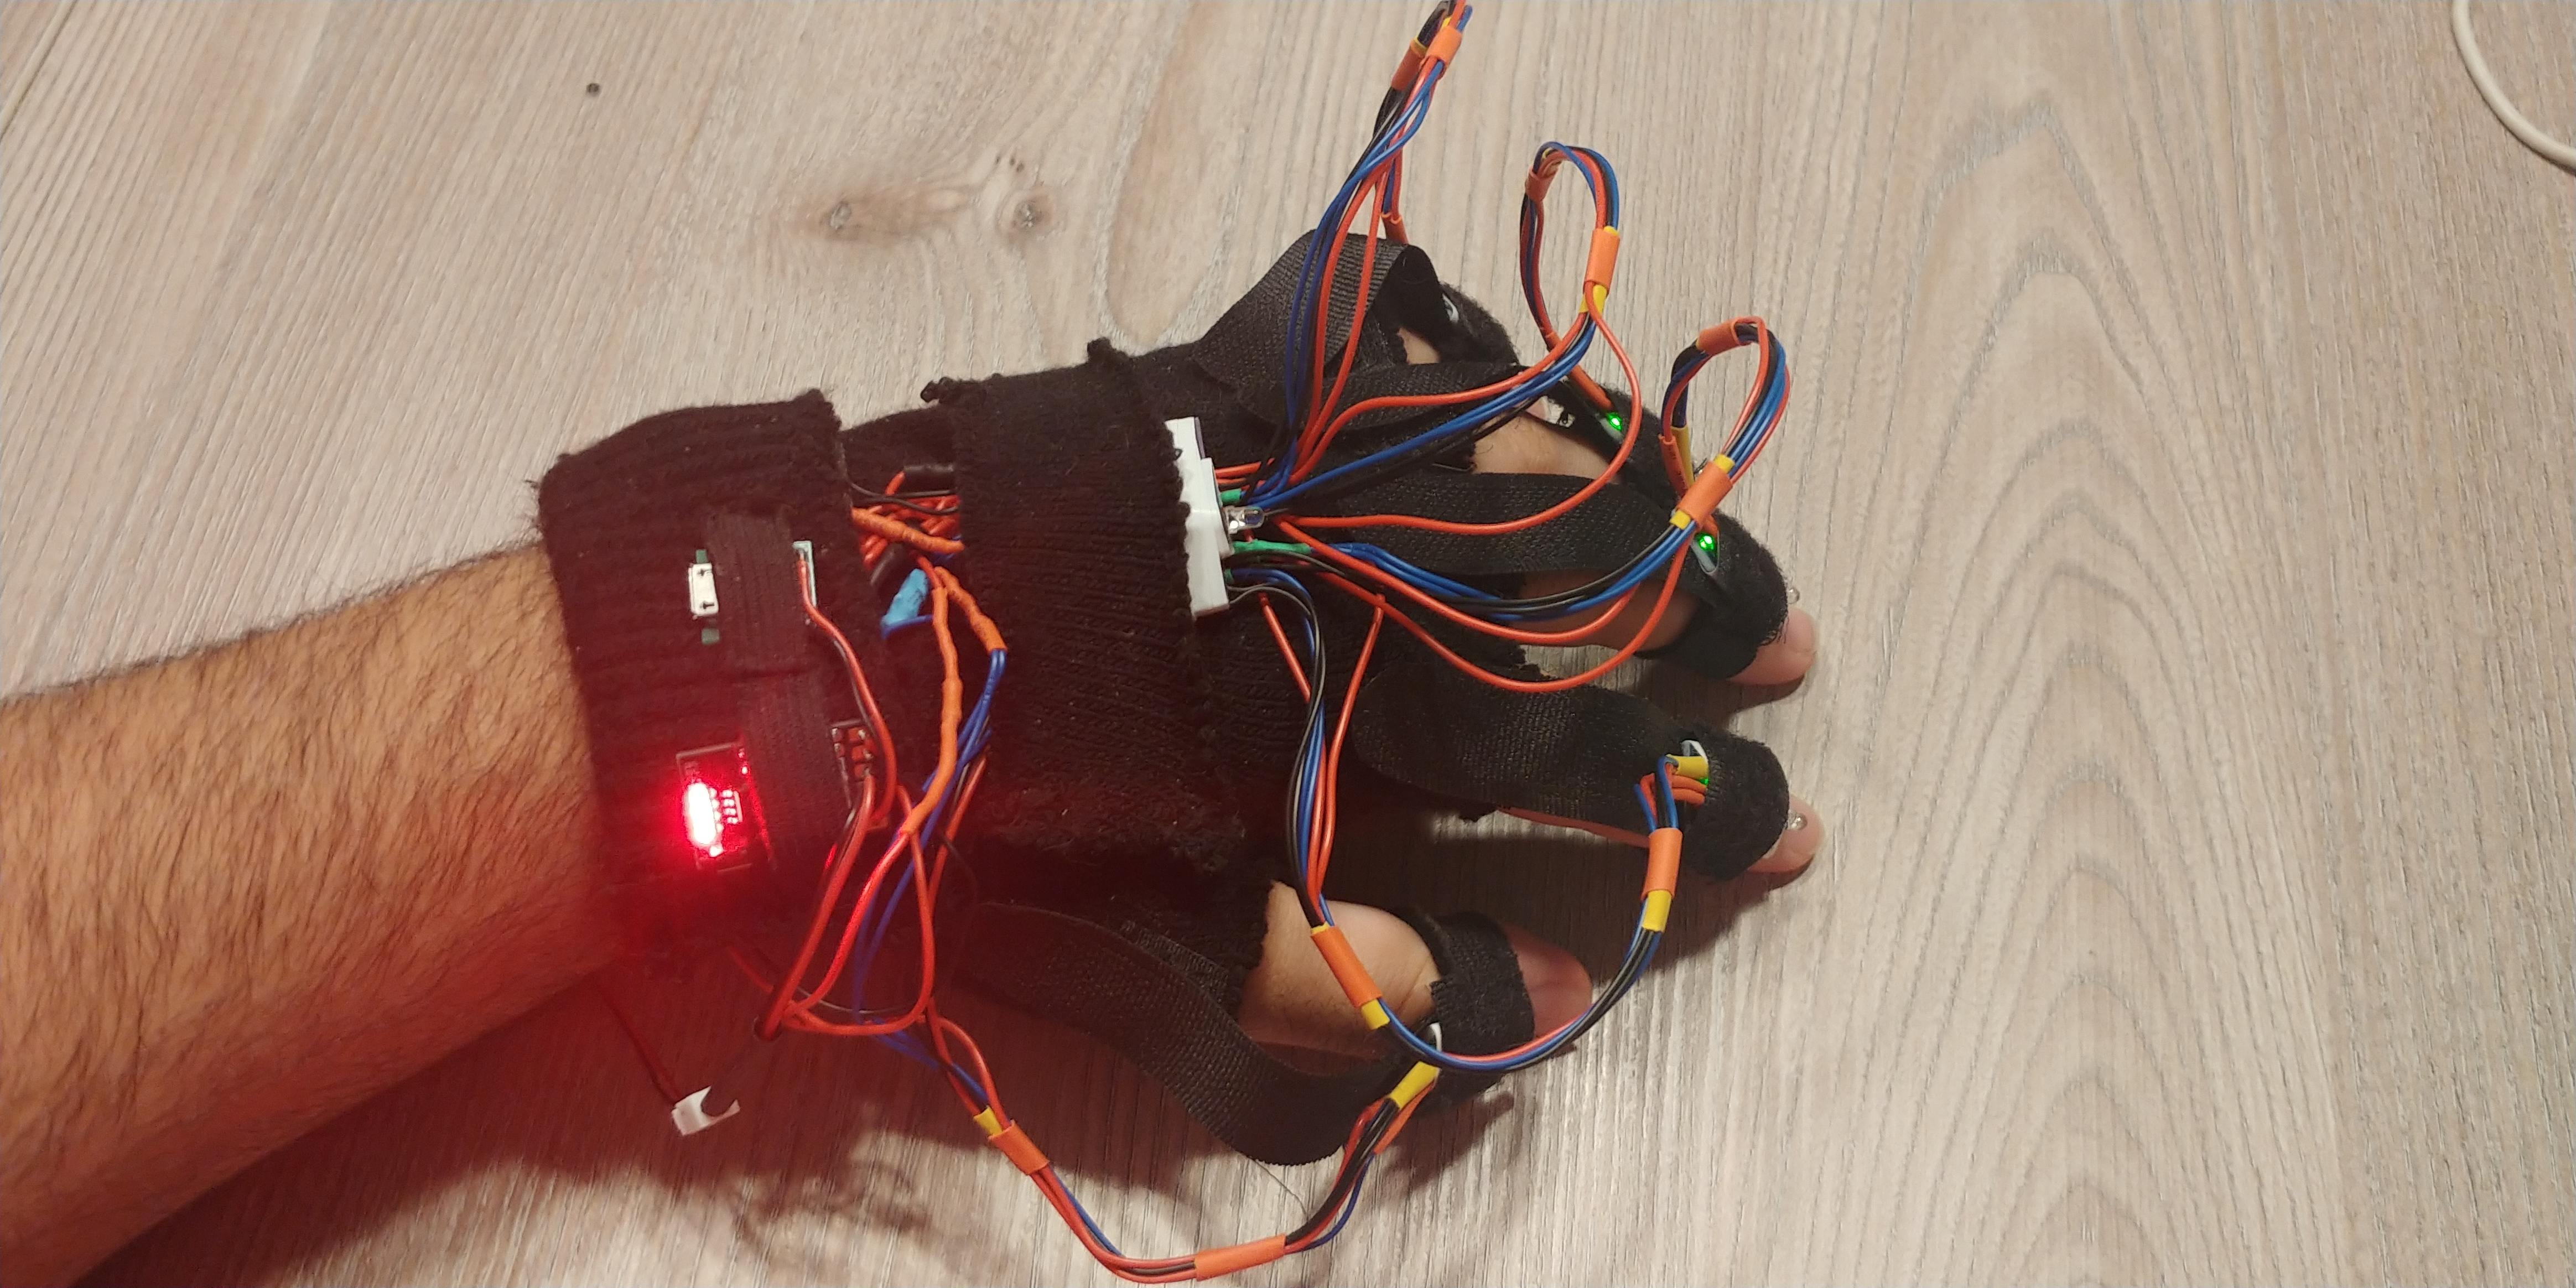
\includegraphics[width=1\columnwidth]{Bachelorarbeit/images/FullView.jpg}
    \caption{Komplett Ansicht des aktiven Datenhandschuh betrieben mit dem eingebauten Akku}
    \label{fig:FullView}
\end{figure}



\section{Datenqualität}
Die Datenqualität unterscheidet sich durch die verschiedene Datenrate stark, dabei hat der MPU-6050 eine Frequenz von $80 Hz$, also das 10-fache vom BMI160.
Wegen der eigentlichen Konstruktion des BMI160, welcher eigentlich für 
niedrigere Leistungskraft, aber genauere Werte spezialisiert. 
Die Rohdaten beider Handschuhe geben im Gesamten eine gute Performanz, wobei der BMI größeres Rauschen \ref{fig:RawData160} misst. 
Die Orientierung konnte mithilfe des Madgwick Filters errechnet werden, jedoch zeigt dieser Drift werte, für beide Datenhandschuhe. 
Der MPU-9259 hatte aber im Gegensatz zu den beiden anderen IMUs den Vorteil einen integrierten Kompass zu haben, durch die Anwendung des Filters in Abhängigkeit der Kompassdaten wurden die Drifts \ref{fig:MagTrueAndFalse} nicht mehr so stark wie ohne die Verwendung des Filters. Diesen somit als Haupt-IMU auf der Mittelhand zu setzen zeigte somit eine starke Stabilisierung der Daten und eine bessere Auswertung der Orientierung.